\section{Introduction}\label{sec:intro}

\IEEEPARstart{C}{ylinder} chess is ordinary chess on a board whose a-file and h-file are joined
\cite{Pritchard}: a white pawn on h4 can capture on a5, a king on a1 can step to h2, and there are no side edges or
corners (Fig.~\ref{fig:ring}). We use combinatorial game theory (CGT) to study its king-and-pawn endgames.

\begin{figure*}[!t]
\centering
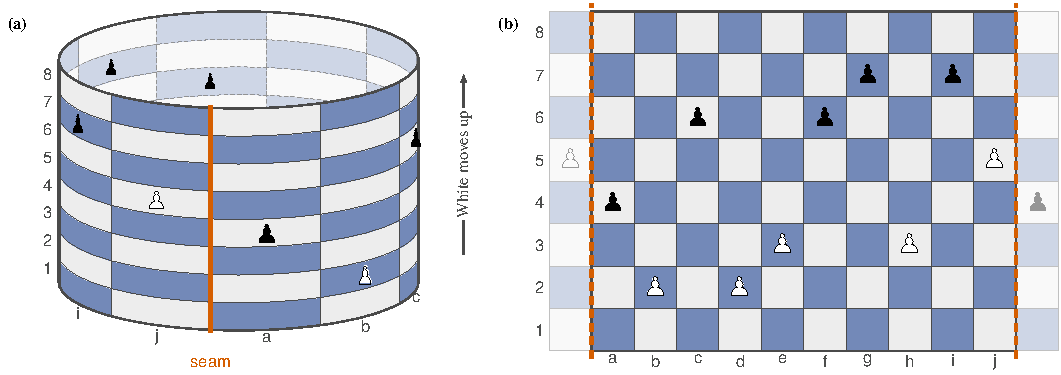
\includegraphics{figures/f1_ring_cylinder_wide.pdf}
\caption{Ring $M_{10}$ on the cylinder $\cyl{10}$. (a)~Perspective view; the seam between files j and a (orange)
faces the viewer, and the far wall is dashed and faded. Only the pawns that can be seen are drawn: 7 of the 10.
(b)~The same position unrolled, with all ten pawns, one per file; file j is next to file a across the dashed
seam, and the faded columns repeat j and a. White moves up. The position has value $\nim{2}$
(Section~\ref{sec:star2-rings}).}
\label{fig:ring}
\end{figure*}

Under normal play the player who cannot move loses; CGT gives each position a value, and a sum of independent
games has the sum of their values \cite{ONAG,WinningWays,Siegel2013}. Chess can be drawn and its kings roam,
yet Elkies \cite{Elkies1996} showed that many pawn endgames split into local fights with exact values, under
two conventions: a passed pawn wins, and is worth a large number $\pm\BIG$; and the kings stand in a mutual
zugzwang, the \emph{tr\'ebuchet}, worth $0$.

The cylinder changes this picture in three ways. There are no rook pawns, and shifting a position sideways
does not change its value. A position with a pawn on every file, a \emph{ring}, has no edge at which to cut
it, and no room for frozen kings, so ring values are values of the pawn-only model. And the corners that decide
mates and fortresses are gone.

Elkies built higher nimbers on large boards from Dawson's pawn game \cite{Elkies2002,Dawson1935}, and
Drummond-Cole built positions of value $\nim{2}$ in chess with the help of pieces other than kings and
pawns~\cite{DrummondCole2005}. We ask whether $\nim{2}$ (Section~\ref{sec:notation}) occurs in a king-and-pawn
endgame on an 8-rank board, the \emph{$\nim{2}$ question}, and whether real chess agrees.

This paper extends an unpublished 2025 study of the basic values\bytheauthor~\cite{Study2025}: we check
every position by computer, correct its errors (Sections~\ref{sec:sums} and~\ref{sec:dawson}) and carry
the analysis on, in the position-by-position format of Wu, Y\"u and Landry~\cite{WuYuLandry2010}. Results carry
labels: \lab{P}, proved here; \lab{S}, proof sketched here, with a full AI-written, AI-refereed proof in the supplement;
\lab{C2}, two separately written programs agree, the second from the rules alone (ours are AI-written; Section~S17); \lab{C1}, one
program; \lab{Conj}, a conjecture. Our contributions are:
\begin{itemize}
\item \emph{Model and kings} (Sections~\ref{sec:rules}, \ref{sec:kings} and~\ref{sec:sums}): a passed-pawn
  test that respects en passant, a cut lemma \lab{P}; conditions (V1)--(V3) under which a frozen tr\'ebuchet gives
  the result of the whole-board pawn game \lab{S}, and (V4) for the $\pm\BIG$ value \lab{S}; a sum-safety
  theorem \lab{S}; and a position showing that checking only the top-level components is not enough \lab{C2}.
\item \emph{Small values} (Sections~\ref{sec:basic}, \ref{sec:atlas} and~\ref{sec:targets}): cylinder-only values come from rings
  \lab{P}; $1/8$ and $\upsec\star$ \lab{C2}, and Tiny~1 \lab{C1}, occur in 10-man positions with a legal pawn
  history.
\item \emph{The $\nim{2}$ question} (Section~\ref{sec:star2}): in the default setting (count rule, e.p.-aware test; Section~\ref{sec:ep}) no $\nim{2}$ has six
  pawns or fewer on ordinary boards of any width, but $\nim{2}$ appears with seven \lab{C2}; in the pawn-only
  model a six-pawn ring suffices on $\cyl{3}$ \lab{C2}, a ring needs ten on $\cyl{7}$ to $\cyl{10}$ \lab{C2}
  and only $n$, one per file, on every $\cyl{n}$ with $n\ge10$ as a whole-board game \lab{S}; on $\cyl{7}$
  some ten-pawn rings are $\nim{3}$ \lab{C2}; $n+1$ pawns give a $\nim{3}$ on $\cyl{11}$ \lab{C2} and on every $\cyl{n}$ with $n\ge12$ \lab{S}.
\item \emph{Real chess} (Section~\ref{sec:real}): with the e.p.-aware test the textbook $\nim{2}$ candidate is not $\nim{2}$, however
  draws are treated \lab{C1}; with queen promotions only and frozen kings, the oracle value of the $1/8$ position is
  exactly $1/8$ \lab{C1}.
\item \emph{Tablebases and Dawson's chess} (Sections~\ref{sec:tb} and~\ref{sec:dawson}): king and rook win only
  2.80\% of cylinder positions, and on the torus, of eight endings, only KRRK and KQRK force mate \lab{C2}; the
  $3\times n$ Dawson cylinder is a first-player win exactly when the $3\times(n-3)$ strip has Grundy value $0$
  \lab{P}.
\item \emph{Engines} (Section~\ref{sec:engines}): in a $233$-position pilot, Stockfish at low depth matches the tablebase least
  often on infinitesimals, significantly less than on hot positions, numbers and switches \lab{C1}.
\end{itemize}
The supplementary material holds the full proofs, further details and the Forsyth--Edwards Notation (FEN) of
the main positions with kings.
